\documentclass[10pt,twocolumn]{article} 

% use the oxycomps style file
\usepackage{oxycomps}

% read references.bib for the bibtex data
\bibliography{references}

% include metadata in the generated pdf file
\pdfinfo{
    /Title (The Ethics of AI Generated Music)
    /Author (William Baron)
}

% set the title and author information
\title{The Ethics of AI Generated Music}
\author{William Baron}
\affiliation{Occidental College}
\email{wbaron@oxy.edu}

\begin{document}

\maketitle

\begin{abstract}
    The field of artificial intelligence is relatively new and as with many new developments, the ethics surrounding it is not very well understood. My comps project aims to write music based on a user inputted chord progression, which while simple on the surface, has lots of ethical implications that cannot all be taken into consideration throughout the duration of this project. Everyone has different needs, and while it is important to address them all and try to make content that is accessible to everyone, I cannot preserve the essence of this project while making it fit everyone's needs.
\end{abstract}

\section{Background}
    My comps project requires a user to input a chord progression and to listen to the output. This will involve interacting with a UI that I've mapped up a draft of here:
    
\begin{figure}[h]
    \centering
    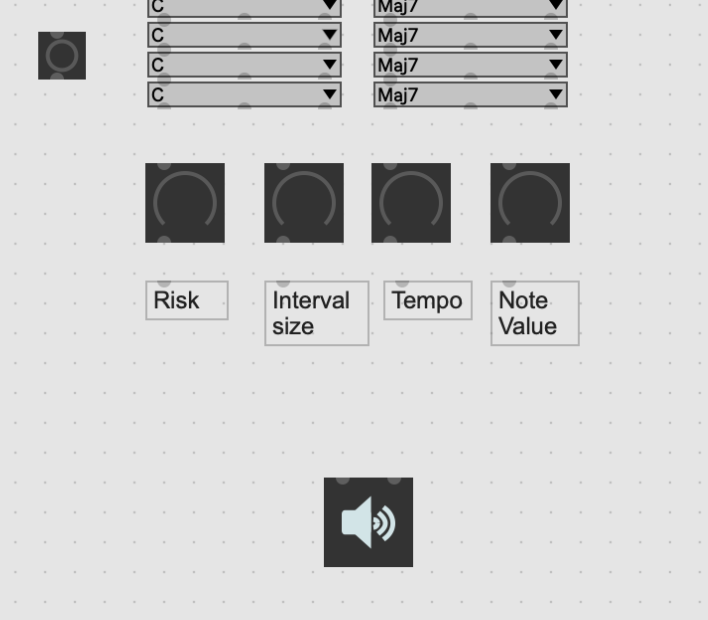
\includegraphics[width=.95\linewidth]{uidraft.png}
    \caption{
        Draft of the UI for my comps project.
    }
    \label{fig:first-page}
\end{figure}

    The user will select the chord root note and the chord quality, adjust the parameters, and press the button to the left of the chord menus to start hearing the output. The output will be aural. The user will hear their four chord loop with the new solo playing over top. The user may then adjust the parameters in real time to hear how the different factors change the content of the solo.

\section{Ethical Challenges}
    Many ethical challenges present themselves upon understanding the goal of my comps project:
    \begin{itemize}
        \item Lack of support for hearing impaired individuals - 
        \newline If someone has difficulty hearing the output of the program, they will miss out on the entirety of my project. It would not be fair to that person if they cannot hear the generated solo since they get no value from interacting with my software.
        \item Lack of support for visually impaired individuals -
        \newline In order to make selections using the various menus and dials, the user has to be able to see them. Without being able to see, there is no way for a user to be able to interact with my project.
        \item Lack of support for individuals with impaired motor functions -
        \newline Similarly to the issues posed in the previous point, if the user cannot use a mouse to use the UI, there is no way for them to use my comps project. 
        \item Western music theory based -
        \newline There are many different schools of thought surrounding the academia and the organization of music. My knowledge of how music works is purely based off of western music theory, which only accounts for a small percentage of the world of music. For example, in some other systems of music theory, micro-tones, or notes between the set of notes used in the western system, are used extensively. Additionally, different scales and chord structures are much more common in other systems which are not represented in my program. For those who are unfamiliar with western music theory, my project will not resonate, nor will the produced solo sound accurate. They may also not understand the requirements of the inputs since they exclusively use the 12 notes used in the equal temperament tuning system used in the west.
        \item Requires some knowledge of music theory -
        \newline If you have no knowledge of western music theory, the program will seem confusing and mysterious. Due to the lack of help and explanation the program provides, users are left to figure out chord progressions on their own. This requires a significant knowledge of music theory and if users input non-diatonic chords, or chords outside of a common key, they might be discouraged by the output when it sounds "wrong".
    \end{itemize}

\section{Addressing the Ethical Challenges}
    \subsection{Lack of Support for Hearing Impaired Individuals}
        If someone cannot hear my project, they cannot enjoy my project. To solve this problem, an option would be integrating some sort of music scoring software to transcribe the output for people to read as they cannot listen. This requires people to be able to read music which reduces the population of people who can use my project significantly, and if someone cannot hear or read music, they cannot interact with my project at all. Another option for the hearing impaired is experiencing music through vibration, however this requires technologies and mediums that I do not want to explore, and the population of people that would need it is too small to warrant exploration (hearing impaired and cannot read music). Addressing these ethical concerns would derail my project since I would have to focus on implementing the sensor technology, and while interesting, I do not have access to these sensors, and their use cases are so niche it would not be worth the implementation.
        \begin{figure}[h]
            \centering
            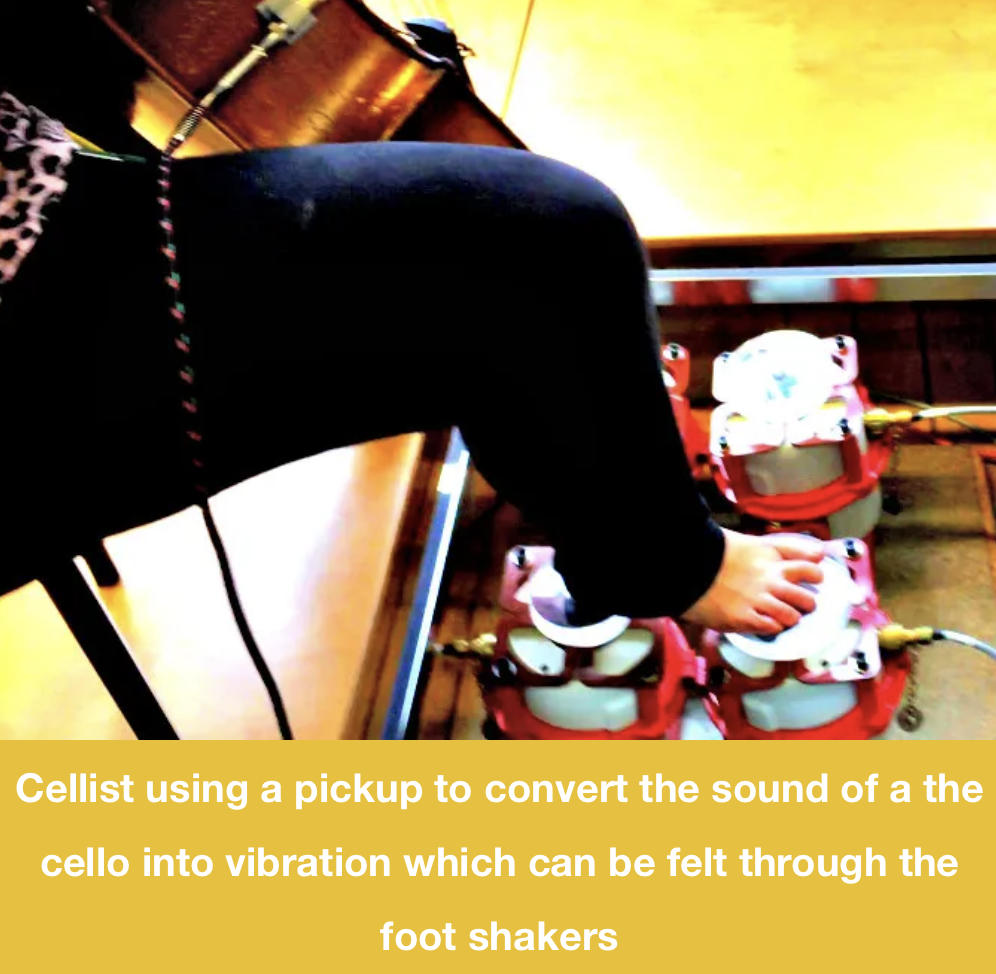
\includegraphics[width=.95\linewidth]{vibes.png}
            \caption{
                The technology for music through vibration\cite{MusicalVibrations}.
            }
            \label{fig:first-page}
        \end{figure}
    
    \subsection{Lack of Support for Visually Impaired Individuals}
        For those who are visually impaired, using the UI will prove difficult. To address these concerns I would need to develop an alternate system of input using tactile responses or sound. The issues with implementing a tactile response system for inputs are the same as the issues with musical vibrations in the previous point, and the issues with creating an interface controlled by sound have a similar cost to reward ratio as the previous point. Solving these challenges creates more challenges for other people. If I create a UI based off of sound, then those who are hearing impaired are affected. If anyone falls under both categories, they simply cannot use my product.
        
    \subsection{Lack of Support for Individuals with Impaired Motor Functions}
        If the user has impaired motor functions, they might not be able to operate the mouse or keyboard which poses similar issues to those in the previous section. An alternate form of input is required, maybe with voice control or eye tracking technology. These issues can be addressed, but not without implementing extensive new technologies, which alongside the other proposed new technologies would require more time than my actual comps project would take. These implementations are simply too much work for the scale of my project and cannot all be done successfully by the comps deadline.
        
    \subsection{Western Music Theory Based}
        If I pitch my project as being able to create a good solo based off of user inputted chord progressions, those who grew up outside of the western sphere of musical influence may not enjoy my output. This is an ethical consideration, however there is always a risk in creating any type of content that someone might not like the result. This should not prevent you from creating the type of content you want to create as long as it doesn't put anyone in danger.
        
    \subsection{Requires Some Knowledge of Music Theory}
        The considerations associated with this section may be important to address in my final project. The majority of people might not be able to create a diatonic chord progression, so a "Help" panel may be incredibly value added to my project. This help section could give a very simple guide on how to create a "good" chord progression and explain why random chord choices sound "bad". This help section could also detail the different parameters and how they affect the output.
        
\section{Conclusion}
    Addressing all ethical concerns for my project is impossible. Even if I had the time to implement the necessary technologies to make my program valuable for every person, these technologies still exclude some percent of the population since some solutions exclude other people. Any population included in the overlap between sensory impaired individuals are still left behind when a solution for hearing impaired individuals requires functioning sight or touch. Additionally, some people growing up with a different style of music is no reason to rework my project. Art is subjective and those with different tastes may be excluded from enjoying my work but that is OK. The population that might not be able to use my project due to a lack of knowledge should be taken into consideration however, since this is a significant percent of the population and it is quite a value added fix.
\printbibliography 

\end{document}